\documentclass[conference]{IEEEtran}
\IEEEoverridecommandlockouts
\usepackage{cite}
\usepackage{amsmath,amssymb,amsfonts}
\usepackage{textcomp}
\usepackage{xcolor}
\usepackage{balance}
\usepackage{booktabs}
\usepackage{float}
\usepackage{graphicx,url}
\usepackage{soulutf8,color}
\usepackage{stfloats}
\usepackage{verbatim}
\usepackage[utf8]{inputenc}
\usepackage[inline]{enumitem}
\usepackage{multirow}
\usepackage{array}
\usepackage{tikz}
\usepackage{hyperref}

\renewcommand{\abstractname}{Resumo}
\renewcommand{\refname}{REFERÊNCIAS}

\begin{document}

\title{Seleção Dinâmica de Algoritmos de Virtual Network Embedding usando XGBoost}

\author{\IEEEauthorblockN{Luis Antonio Momm Duarte}
\IEEEauthorblockA{\textit{Programa de Pós-Graduação em Computação Aplicada} \\
\textit{Universidade do Estado de Santa Catarina}\\
Joinville, Brasil \\
luis.duarte@edu.udesc.br}
\and
\IEEEauthorblockN{Adriano Fiorese}
\IEEEauthorblockA{\textit{Department of Computer Science} \\
\textit{Santa Catarina State University}\\
Joinville, Brazil \\
adriano.fiorese@udesc.br}
}

\maketitle

\begin{abstract}
A crescente demanda por virtualização de redes em infraestruturas modernas de computação em nuvem tornou o \textit{Virtual Network Embedding} (VNE) uma área crítica de pesquisa. Embora numerosos algoritmos de VNE tenham sido propostos, nenhum algoritmo único apresenta desempenho consistentemente superior em todos os cenários. É proposta uma abordagem inovadora que utiliza aprendizado de máquina, especificamente \textit{XGBoost}, para selecionar inteligentemente o algoritmo mais apropriado para cada requisição de rede virtual recebida. Resultados experimentais demonstram que o seletor dinâmico alcança 93,33\% de acurácia na predição do melhor algoritmo, com taxa de aceitação de 43,33\% e tempo médio de resolução de 5,63s, ficando apenas 1,67 pontos percentuais abaixo do oráculo teórico ótimo. O modelo identifica topologia e tamanho relativo da VNR como os fatores mais importantes para seleção de algoritmo, demonstrando melhorias estatisticamente significativas em relação a algoritmos baseline individuais.
\end{abstract}

\begin{IEEEkeywords}
Virtual Network Embedding, Machine Learning, XGBoost, Network Virtualization, Algorithm Selection
\end{IEEEkeywords}

%===================================================================

\section{Introdução}
\label{sec:Intro}

A crescente demanda por virtualização de redes em infraestruturas modernas de computação em nuvem tornou o problema de \textit{Virtual Network Embedding} (VNE) uma área crítica de pesquisa. O VNE aborda o problema de mapear requisições de redes virtuais (\textit{Virtual Network Requests} - VNRs) sobre a infraestrutura de rede física, satisfazendo restrições de recursos e otimizando objetivos específicos como taxa de aceitação, utilização de recursos e consumo de energia.

Na última década, numerosos algoritmos de VNE foram propostos, variando desde métodos exatos baseados em Programação Inteira Mista (MIP) até abordagens heurísticas e meta-heurísticas. Algoritmos exatos como MIP garantem soluções ótimas mas sofrem com problemas de escalabilidade e altos custos computacionais. Métodos heurísticos como \textit{D-Rounding} e \textit{RW-Rank-BFS} oferecem tempos de execução mais rápidos, mas podem produzir alocações subótimas. Abordagens meta-heurísticas como \textit{Genetic Algorithms} (GA), \textit{Particle Swarm Optimization} (PSO) e \textit{Monte Carlo Tree Search} (MCTS) tentam balancear qualidade da solução e tempo de execução, porém seu desempenho varia significativamente dependendo das características da instância do problema.

Apesar da extensa pesquisa em algoritmos de VNE, um desafio fundamental permanece: nenhum algoritmo único apresenta desempenho consistentemente superior em todos os cenários de rede e características de carga de trabalho.
Este fenômeno, conhecido como o teorema \("\)No Free Lunch\("\) em otimização, sugere que a escolha do melhor algoritmo é inerentemente dependente do problema.
Rice~\cite{rice1976algorithm} formalizou o problema de seleção de algoritmos, estabelecendo que características da instância determinam qual método será mais eficaz.
Nessa linha, trabalhos como \textit{SATzilla}~\cite{xu2012satzilla} demonstraram o sucesso de seleção de algoritmos em portfólio em problemas de satisfabilidade, motivando aplicações similares em VNE.
Abordagens tradicionais para implantação de VNE tipicamente selecionam um único algoritmo "bala de prata" para todas as requisições recebidas, independentemente de suas características ou do estado atual da rede física.
Esta estratégia única para todos os casos falha em explorar os pontos fortes de diferentes algoritmos para diferentes cenários.

Por exemplo, VNRs pequenas com baixas demandas de recursos podem ser eficientemente tratadas por heurísticas rápidas, enquanto requisições maiores e mais complexas poderiam se beneficiar de métodos exatos ou meta-heurísticas. Similarmente, o estado atual da rede física, como fragmentação de recursos, capacidade disponível e topologia da rede, influencia significativamente qual algoritmo apresentará melhor desempenho.

Propõe-se uma abordagem para VNE que utiliza aprendizado de máquina, especificamente \textit{XGBoost} (\textit{Extreme Gradient Boosting}), para selecionar inteligentemente o algoritmo mais apropriado para cada requisição de rede virtual recebida. Ao invés de um único algoritmo, o método proposto analisa as características de cada VNR e o estado atual da rede física para predizer qual algoritmo produzirá os melhores resultados em termos de taxa de aceitação e tempo de solução. Esta estratégia de seleção adaptativa visa combinar os pontos fortes de múltiplos algoritmos, potencialmente alcançando melhor desempenho geral do que qualquer método individual.

As principais contribuições deste trabalho são:

\begin{itemize}
    \item Um conjunto diverso de simulações utilizando a plataforma \textit{ViRNE}, executando sete diferentes algoritmos de VNE (exatos, heurísticos e meta-heurísticos) em topologias \textit{Tree} e \textit{Fat-Tree} com parâmetros variados e diferentes características de carga, resultando em 8000 VNRs únicas para treinamento.

    \item Uma metodologia de engenharia de \textit{features} que captura 17 características relevantes das VNRs e estados da rede física, incluindo métricas topológicas, demandas de recursos, capacidade disponível e indicadores de utilização.

    \item Um modelo de classificação baseado em \textit{XGBoost} com otimização de hiperparâmetros via \textit{Grid Search}, alcançando 93,33\% de acurácia e \textit{F1-score} ponderado de 92,36\% na predição do melhor algoritmo para cada requisição.

    \item Uma avaliação experimental comparando a abordagem de seleção dinâmica contra sete algoritmos individuais e um oráculo teórico, demonstrando que o \textit{XGBoost} alcança desempenho quase ótimo com apenas 1,67\% de diferença em taxa de aceitação.

    \item Análise de importância de \textit{features} revelando que topologia e tamanho relativo da VNR são os fatores mais críticos para seleção de algoritmo, permitindo interpretação sobre o processo de decisão.

    \item Reprodutibilidade completa com código fonte, dados de simulação e modelos treinados disponibilizados publicamente.
\end{itemize}

O restante deste artigo está organizado da seguinte forma: a Seção~\ref{sec:RefTeo} apresenta o referencial teórico necessário para compreensão do problema de VNE e técnicas de aprendizado de máquina usando árvores de decisão, como o \textit{XGBoost}; a Seção~\ref{sec:Proposal} descreve a metodologia proposta, incluindo o processo de geração de dados de simulação, extração de \textit{features}, treinamento do modelo \textit{XGBoost} e estratégia de avaliação; a Seção~\ref{sec:Results} apresenta os resultados experimentais, analisando o desempenho do seletor dinâmico em comparação com algoritmos \textit{baseline}; finalmente, a Seção~\ref{sec:Conclusion} conclui o artigo e delineia direções futuras de pesquisa.

\section{Referencial Teórico}
\label{sec:RefTeo}

\subsection{\textit{Virtual Network Embedding}}

\textit{Virtual Network Embedding} (VNE) é o processo de mapear requisições de redes virtuais sobre uma infraestrutura de rede física compartilhada, respeitando restrições de capacidade de recursos. Uma requisição de rede virtual $G_v = (N_v, L_v)$ consiste em um conjunto de nós virtuais $N_v$ e enlaces virtuais $L_v$, em que cada nó e enlace possui demandas de recursos específicas (CPU, memória, banda). A rede física $G_p = (N_p, L_p)$ fornece os recursos computacionais e de rede para hospedar as VNRs.

O problema de VNE pode ser decomposto em dois subproblemas: (1) mapeamento de nós virtuais para nós físicos e (2) mapeamento de enlaces virtuais para caminhos na rede física. O objetivo é maximizar métricas como taxa de aceitação de VNRs, utilização de recursos e receita do provedor, enquanto minimiza custos operacionais e tempo de processamento.

O VNE é conhecido por ser NP-difícil mesmo em casos simplificados \cite{vnboost}, motivando o desenvolvimento de diversas classes de algoritmos:

\textbf{Algoritmos Exatos}: Formulações baseadas em \textit{Programação Linear Inteira} (ILP) ou \textit{Programação Inteira Mista} (MIP) garantem soluções ótimas mas possuem complexidade exponencial. São práticos apenas para instâncias pequenas devido ao tempo de resolução proibitivo para larga escala.

\textbf{Heurísticas}: Algoritmos gulosos que tomam decisões locais baseadas em \textit{rankings} de nós ou estratégias de busca. Exemplos incluem \textit{NodeRank}, \textit{D-Rounding} e algoritmo de busca de caminho. Oferecem tempo de execução rápido mas qualidade de solução variável.

\textbf{Meta-heurísticas}: Técnicas de busca estocástica como algoritmos genéticos (GA), \textit{Particle Swarm Optimization} (PSO), \textit{Simulated Annealing} (SA) e \textit{Monte Carlo Tree Search} (MCTS). Balanceiam exploração do espaço de busca, oferecendo \textit{trade-off} entre qualidade e tempo.

\subsection{XGBoost}

\textit{XGBoost} (\textit{Extreme Gradient Boosting})~\cite{chen2016xgboost} é um algoritmo de aprendizado de máquina, de código aberto, baseado em conjunto de modelos de árvores de decisão que utiliza a técnica de \textit{gradient boosting}. O algoritmo constrói modelos preditivos de forma iterativa, em que cada nova árvore corrige os erros das árvores anteriores.

O \textit{XGBoost} otimiza uma função objetivo que combina uma função de perda (\textit{loss function}) com termos de regularização para prevenir \textit{overfitting}:

\begin{itemize}
    \item \textbf{Desempenho}: Implementação eficiente com otimizações como paralelização.
    \item \textbf{Regularização}: Penalização de complexidade do modelo (L1 e L2) previne \textit{overfitting}.
    \item \textbf{Operação de Dados Esparsos}: Tratamento eficiente de valores faltantes
    \item \textbf{Interpretabilidade}: Métricas de importância de \textit{features} facilitam análise do modelo
    \item \textbf{Flexibilidade}: Suporta classificação multiclasse, regressão e \textit{ranking}
\end{itemize}

Para problemas de classificação multiclasse, o \textit{XGBoost} utiliza \textit{softmax} para computar probabilidades de classe e otimiza a função de \textit{cross-entropy}.
Além disso, o algoritmo é bastante utilizado em estudos de aprendizado de máquina, fornecendo ampla documentação e bibliotecas prontas para seu uso, motivando
a escolha.

\subsection{Seleção de Algoritmos}

A seleção de algoritmos pode ser formulada como um problema de aprendizado supervisionado, onde o objetivo é aprender uma função de mapeamento $f: \mathcal{F} \rightarrow \mathcal{A}$ que mapeia \textit{features} de instância $\mathcal{F}$ para o melhor algoritmo $\mathcal{A}$.

O \textit{framework} de seleção de algoritmos pode ser aplicado ao contexto de VNE da seguinte forma:

\begin{itemize}
    \item \textbf{Espaço de Problemas (\textit{Problem Space})}: consiste no conjunto de todas as possíveis requisições de redes virtuais (VNRs), caracterizadas por diferentes tamanhos (número de nós e enlaces), topologias (estruturas de grafo variadas) e demandas de recursos (CPU, memória, banda).

    \item \textbf{Espaço de Algoritmos (\textit{Algorithm Space})}: compreende o portfólio de algoritmos de VNE disponíveis, incluindo métodos exatos (MIP), heurísticas (\textit{D-Rounding}, \textit{RW-Rank-BFS}) e meta-heurísticas (GA, PSO, MCTS, SA).

    \item \textbf{Espaço de \textit{Features} (\textit{Feature Space})}: conjunto de características mensuráveis que descrevem cada instância do problema, capturando propriedades da VNR (tamanho, conectividade, demandas) e estado atual da rede física (utilização de recursos, capacidade disponível, número de VNRs ativas).

    \item \textbf{Espaço de Desempenho (\textit{Performance Space})}: Métricas utilizadas para avaliar a qualidade das soluções, incluindo taxa de aceitação de VNRs, tempo de resolução, utilização de recursos e receita gerada.
\end{itemize}

O objetivo do seletor de algoritmos é aprender a função de mapeamento que, dado um vetor de \textit{features} extraído de uma nova VNR e do estado da rede física, seleciona o algoritmo que maximizará as métricas de desempenho desejadas.

\subsection{ViRNE: Plataforma de \textit{Benchmark}}\label{subsec:virne:-plataforma-de-benchmark}

Para realizar a experimentação e coleta de dados necessários ao treinamento do seletor de algoritmos, foi utilizado o \textit{ViRNE}\cite{virne}, uma plataforma unificada de \textit{benchmark} para \textit{Virtual Network Embedding}.
O ViRNE fornece uma infraestrutura completa e padronizada para avaliação e comparação justa de diferentes algoritmos de VNE.

A plataforma oferece implementações de diversos algoritmos de VNE (exatos, heurísticos e meta-heurísticos), permitindo a execução de experimentos reproduzíveis com controle rigoroso sobre parâmetros de simulação.
Além disso, o \textit{ViRNE} inclui funcionalidades de \textit{logging} detalhado e extração de métricas, facilitando a coleta das \textit{features} e resultados necessários para o treinamento de modelos de aprendizado de máquina.

A escolha do \textit{ViRNE} como plataforma de experimentação é motivada por: (1) reprodutibilidade dos experimentos através de configurações padronizadas; (2) diversidade de algoritmos implementados, permitindo comparação abrangente; (3) facilidade de extração de dados para \textit{machine learning}; e (4) suporte a diferentes topologias de rede e cenários de carga.

\section{Metodologia}
\label{sec:Proposal}

Esta seção descreve a metodologia proposta para seleção dinâmica de algoritmos VNE usando \textit{XGBoost}, incluindo o processo de geração de simulações, engenharia de \textit{features}, treinamento do modelo e estratégia de avaliação.

\subsection{Visão Geral da Abordagem}

A abordagem proposta consiste em quatro etapas principais:

\begin{enumerate}
    \item \textbf{Coleta de Dados}: Executar múltiplos algoritmos VNE em topologias variadas para coletar dados de desempenho
    \item \textbf{Engenharia de \textit{Features}}: Extrair características relevantes das VNRs e estado da rede física
    \item \textbf{Treinamento do Modelo}: Otimizar hiperparâmetros do \textit{XGBoost} e treinar classificador multiclasse
    \item \textbf{Predição \textit{Online}}: Para cada nova VNR, predizer o melhor algoritmo e executá-lo
\end{enumerate}

O fluxo operacional do sistema é o seguinte: quando uma nova VNR chega, suas características (número de nós, demandas de recursos, topologia) e o estado atual da rede física (utilização de recursos, número de VNRs ativas) são extraídos como \textit{features}.
O modelo \textit{XGBoost} treinado prediz qual algoritmo deve ser utilizado. O algoritmo selecionado é então executado para tentar mapear a VNR sobre a rede física.

\subsection{Geração de dados de simulações}

Os dados foram coletados utilizando a plataforma \textit{ViRNE}, executando simulações de VNE com sete diferentes algoritmos em duas topologias de \textit{datacenter}: árvore binária e \textit{fat-tree}. Os algoritmos avaliados incluem:

\begin{itemize}
    \item \textbf{MIP}: \textit{Mixed Integer Programming} (método exato)
    \item \textbf{GA-Meta}: \textit{Genetic Algorithm} com \textit{meta-learning}
    \item \textbf{PSO-Meta}: \textit{Particle Swarm Optimization} com \textit{meta-learning}
    \item \textbf{SA-Meta}: \textit{Simulated Annealing} com \textit{meta-learning}
    \item \textbf{MCTS}: \textit{Monte Carlo Tree Search}
    \item \textbf{PL-Rank}: \textit{PageRank-based heuristic}
    \item \textbf{RW-Rank-BFS}: \textit{Random Walk Rank} com \textit{Breadth-First Search}
    \item \textbf{D-Round}: \textit{Deterministic Rounding heuristic}
\end{itemize}

As topologias utilizadas foram:

\begin{itemize}
    \item \textbf{\textit{Tree}}: Topologia hierárquica em árvore binária com 32 \textit{hosts} (nós folha) e 31 \textit{switches} internos, totalizando 63 nós
    \item \textbf{\textit{Fat-Tree}}: Topologia de \textit{datacenter} com k=4 (16 servidores \textit{hosts}, 20 \textit{switches}), totalizando 36 nós
\end{itemize}

\textbf{Pré-processamento das Topologias:} As topologias físicas foram pré-processadas para distinguir nós de roteamento (\textit{switches}) de nós computacionais (\textit{hosts}). Todos os \textit{switches} internos receberam CPU=0, representando sua função exclusiva de roteamento, enquanto os \textit{hosts} (nós folha na \textit{Tree} e servidores na \textit{Fat-Tree}) mantiveram recursos computacionais normais (CPU entre 50-100 unidades). Este pré-processamento garante que as VNRs sejam mapeadas apenas em nós com capacidade computacional real.

Para cada combinação de algoritmo e topologia, foram executadas dez repetições com diferentes sementes aleatórias para garantir significância estatística. Cada simulação gerou aproximadamente cem VNRs, totalizando 11.672 execuções de algoritmos. Após deduplicação (removendo múltiplas execuções da mesma VNR), foram obtidas oito mil VNRs únicas para treinamento.

Os parâmetros de geração de VNRs foram:

\begin{itemize}
    \item Número de nós virtuais: 2 a 10 nós
    \item Probabilidade de conexão entre nós: 50\%
    \item Demanda de CPU/recursos de nós: [0, 20] unidades
    \item Demanda de banda de enlaces: [0, 50] unidades
    \item Tempo de vida: distribuição exponencial com média de 500 unidades
    \item Taxa de chegada: processo de Poisson variável
\end{itemize}

A rede física possui, distribuída de maneira uniforme:

\begin{itemize}
    \item Capacidade de nós: [50, 100] unidades de CPU
    \item Capacidade de enlaces: [50, 100] unidades de banda
\end{itemize}

\subsection{Engenharia de \textit{Features}}

Um dos aspectos mais críticos do trabalho foi a definição de \textit{features} que capturam características relevantes das VNRs e estado da rede física. O conjunto final de \textit{features} inclui 17 características divididas em quatro categorias:

\textbf{Características da VNR} (nove \textit{features}):
\begin{itemize}
    \item \texttt{v\_net\_num\_nodes}: Número de nós virtuais
    \item \texttt{v\_net\_num\_edges}: Número de enlaces virtuais
    \item \texttt{v\_net\_size\_ratio}: Razão entre tamanho da VNR e rede física
    \item \texttt{v\_net\_demand\_per\_node}: Demanda média por nó
    \item \texttt{v\_net\_demand\_per\_enlace}: Demanda média por link
    \item \texttt{v\_net\_connectivity}: Densidade de conexões (edges/nodes)
    \item \texttt{v\_net\_total\_demand}: Demanda total de recursos
    \item \texttt{v\_net\_node\_to\_enlace\_demand\_ratio}: Razão entre demanda de nós e links
    \item \texttt{v\_net\_lifetime}: Tempo de vida esperado da VNR
\end{itemize}

\textbf{Estado da Rede Física} (quatro \textit{features}):
\begin{itemize}
    \item \texttt{p\_net\_available\_resource}: Total de recursos disponíveis
    \item \texttt{p\_net\_node\_util}: Utilização média dos nós físicos
    \item \texttt{p\_net\_enlace\_util}: Utilização média dos links físicos
    \item \texttt{p\_net\_overall\_util}: Utilização geral da rede
\end{itemize}

\textbf{Estado do Sistema} (três \textit{features}):
\begin{itemize}
    \item \texttt{inservice\_count}: Número de VNRs atualmente ativas
    \item \texttt{system\_load}: Carga normalizada do sistema
    \item \texttt{num\_running\_p\_net\_nodes}: Número de nós físicos ativos
\end{itemize}

\textbf{Contexto} (uma \textit{feature}):
\begin{itemize}
    \item \texttt{topology\_encoded}: Tipo de topologia (tree vs fat-tree)
\end{itemize}

\subsection{Treinamento do Modelo \textit{XGBoost}}

O \textit{dataset} de oito mil VNRs foi dividido em três conjuntos:
\begin{itemize}
    \item \textbf{Treinamento}: 5600 VNRs (70\%)
    \item \textbf{Validação}: 1200 VNRs (15\%)
    \item \textbf{Teste}: 1200 VNRs (15\%)
\end{itemize}

Os hiperparâmetros do \textit{XGBoost} foram otimizados via \textit{Grid Search} com validação cruzada de quatro \textit{folds}. O espaço de busca incluiu:

\begin{itemize}
    \item \texttt{max\_depth}: [3, 5, 7, 10]
    \item \texttt{learning\_rate}: [0.01, 0.05, 0.1, 0.2]
    \item \texttt{n\_estimators}: [50, 100, 200, 300]
    \item \texttt{subsample}: [0.6, 0.8, 1.0]
    \item \texttt{colsample\_bytree}: [0.6, 0.8, 1.0]
\end{itemize}

A melhor configuração encontrada foi:
\begin{itemize}
    \item \texttt{max\_depth}: 7
    \item \texttt{learning\_rate}: 0.1
    \item \texttt{n\_estimators}: 200
    \item \texttt{subsample}: 0.8
    \item \texttt{colsample\_bytree}: 0.8
\end{itemize}

O modelo foi treinado para classificação multiclasse com objetivo de maximizar o \textit{F1-score} ponderado. O tempo total de treinamento foi de aproximadamente trinta segundos em um \textit{MacBook Air} com processador \textit{Apple} M1 (2024) e 16GB de RAM.

\subsection{Métricas de Avaliação}

O desempenho do seletor dinâmico foi avaliada usando múltiplas métricas:

\textbf{Métricas de Classificação}:
\begin{itemize}
    \item \textbf{Acurácia}: Proporção de predições corretas
    \item \textbf{Matriz de Confusão}: Análise de erros de classificação
\end{itemize}

\textbf{Métricas de Desempenho do Seletor}:
\begin{itemize}
    \item \textbf{Taxa de Aceitação}: Porcentagem de VNRs aceitas com sucesso
    \item \textbf{Tempo Médio de Resolução}: Tempo médio para processar uma VNR
    \item \textbf{Diferença para o Oráculo}: Diferença de desempenho comparado ao melhor algoritmo possível (oráculo)
\end{itemize}

O \textbf{oráculo} representa um limite teórico superior, selecionando sempre o algoritmo que produziu o melhor resultado para cada VNR específica (conhecimento perfeito do futuro). Comparar contra o oráculo quantifica o "arrependimento" da estratégia de seleção.

\section{Resultados Experimentais}
\label{sec:Results}

Esta seção apresenta os resultados experimentais do seletor dinâmico de algoritmos \textit{XGBoost}, incluindo desempenho de classificação, comparação com \textit{baselines} e análise de importância de \textit{features}.

\subsection{Desempenho de Classificação}

\begin{itemize}
    \item \textbf{Acurácia}: 93,33\%
    \item \textbf{\textit{F1-Score} Ponderado}: 92,36\%
\end{itemize}

\subsection{Importância das \textit{Features}}

A análise de importância de \textit{features} (Figura~\ref{fig:feature_importance}) revela os fatores mais críticos para seleção de algoritmos:

\begin{figure}[H]
    \centering
    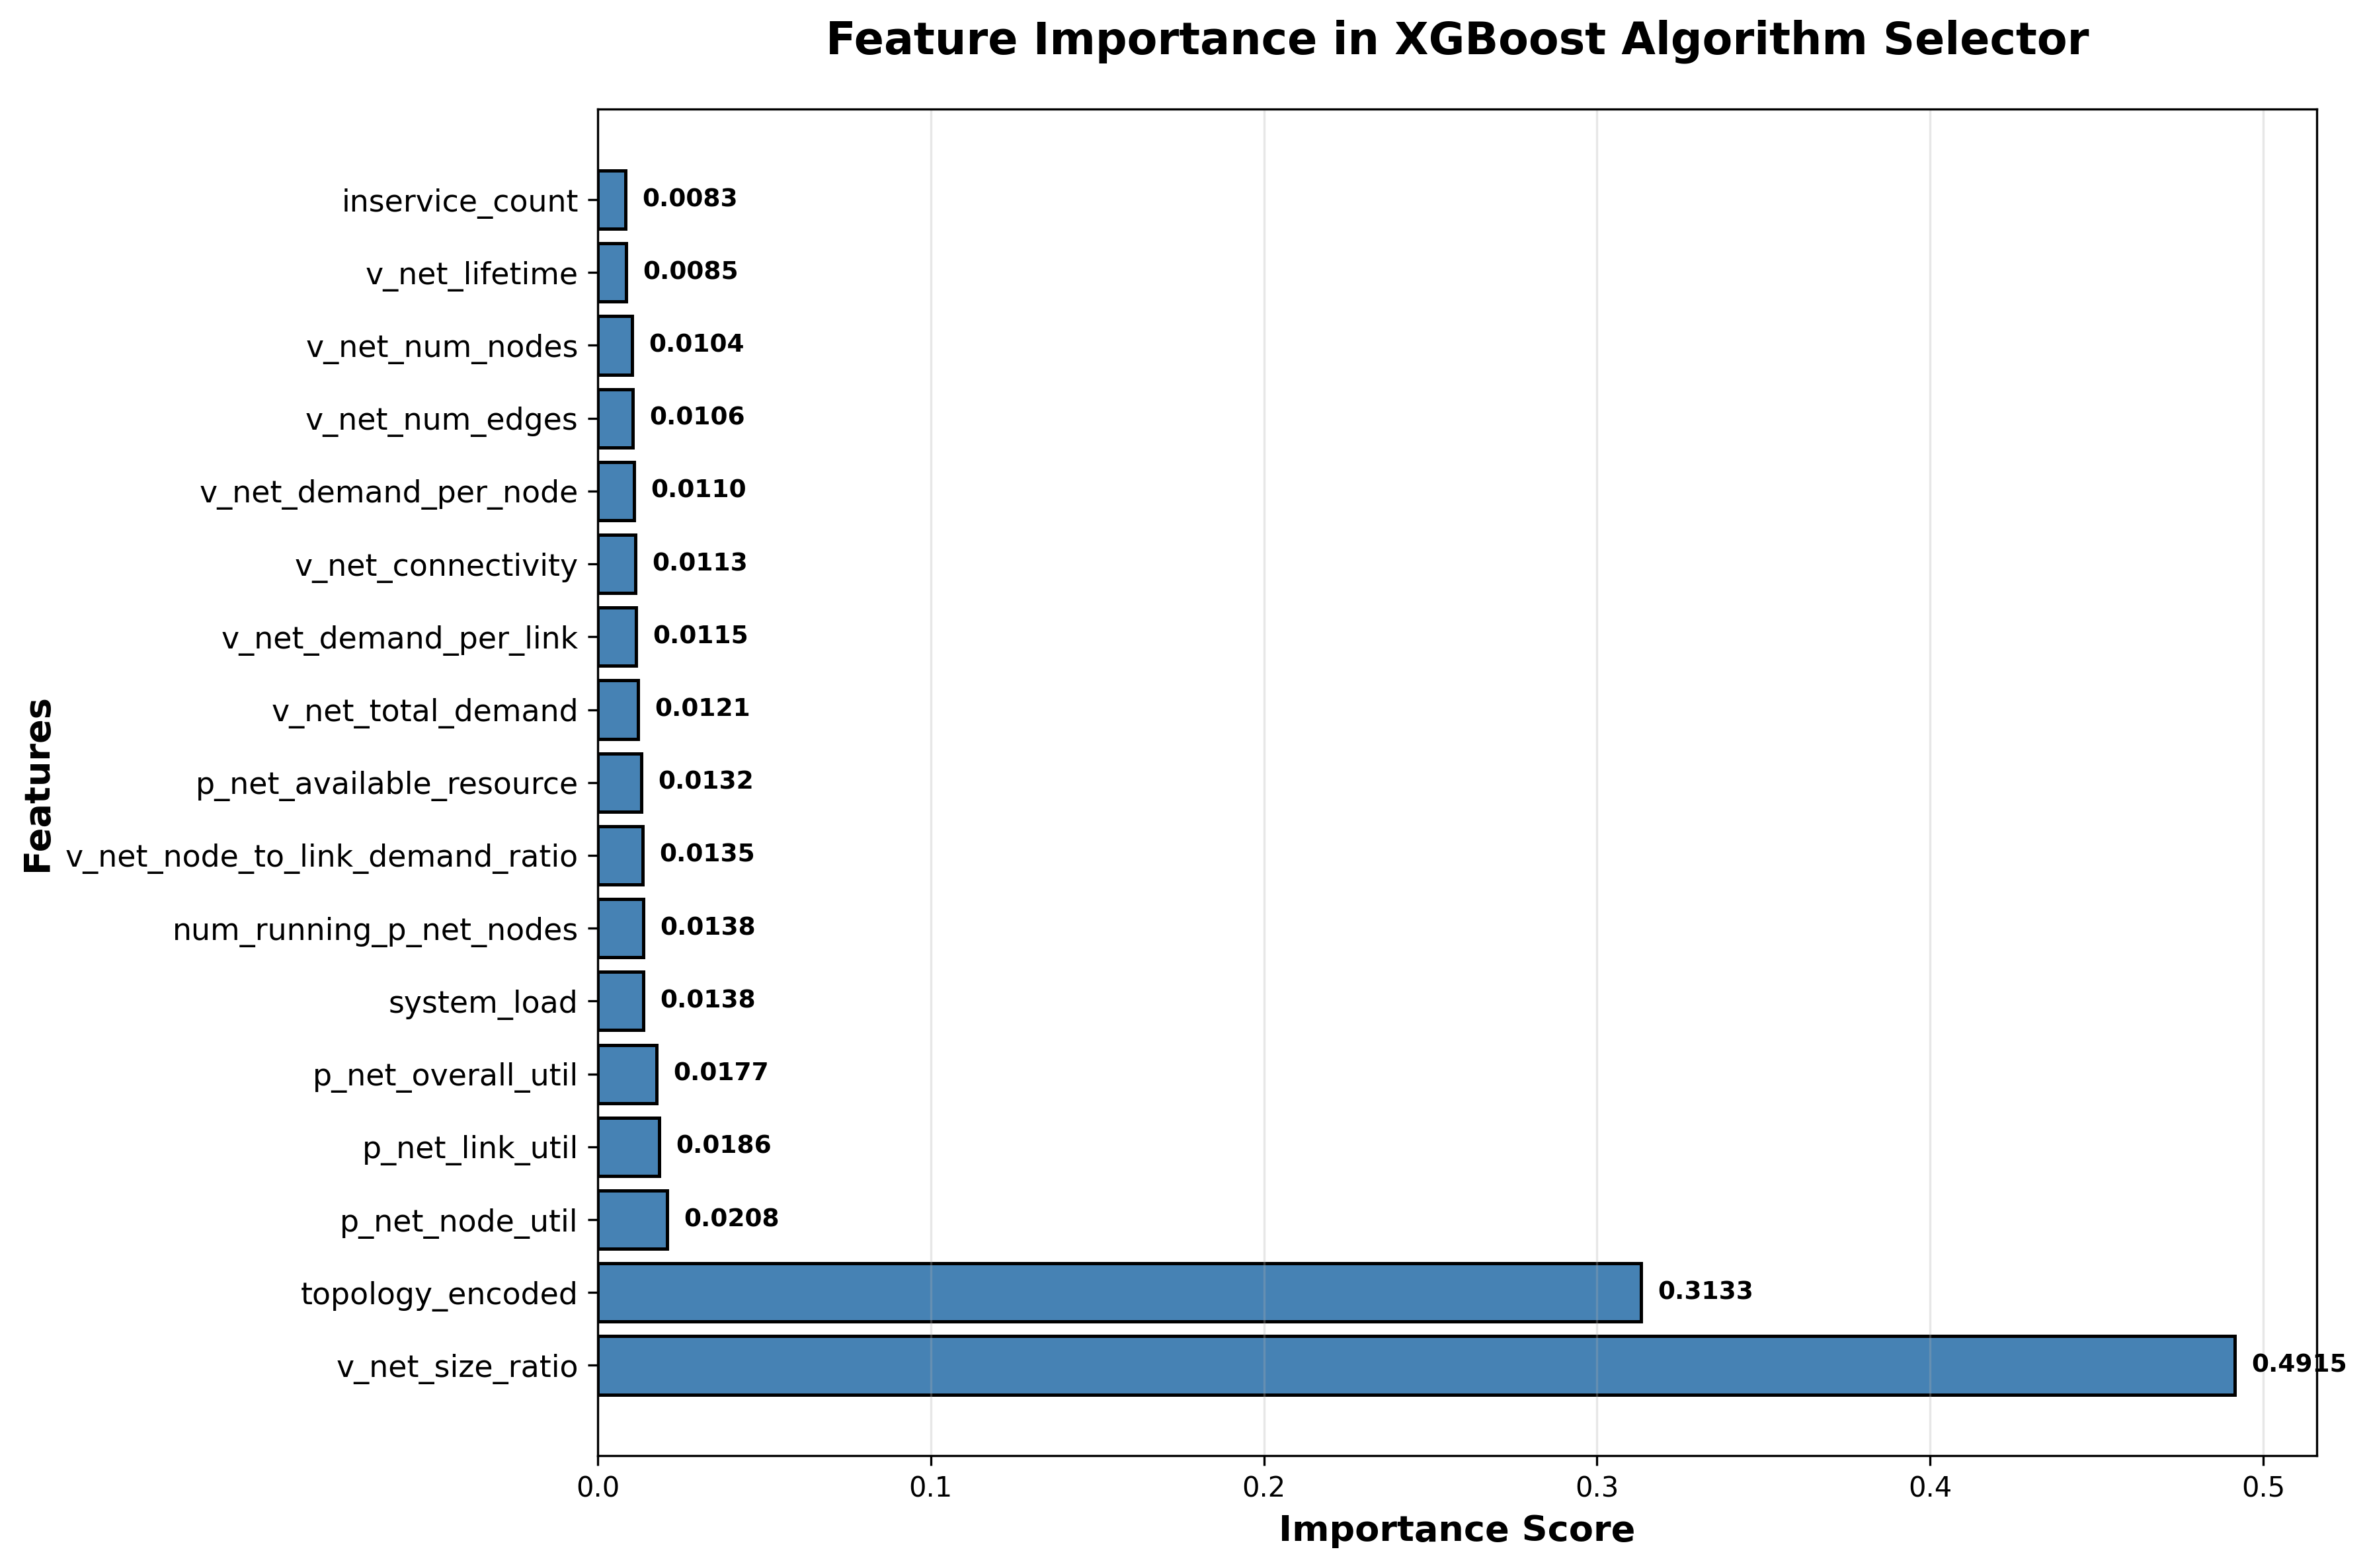
\includegraphics[width=\linewidth]{feature_importance.png}
    \caption{Importância das \textit{Features} no Modelo \textit{XGBoost}}
    \label{fig:feature_importance}
\end{figure}

\textbf{Intuição Chave}: Tamanho relativo da VNR (49,15\%) e topologia (31,33\%) são os fatores dominantes para seleção de algoritmo, representando juntos 80,48\% da importância total.
O tamanho relativo da VNR indica a complexidade do problema de mapeamento, enquanto a topologia física determina a adequação estrutural de diferentes estratégias.
\textit{Features} de utilização da rede física (nós, enlaces e geral) têm importância secundária (dois a três por cento cada), mas ainda relevante para decisões em cenários de alta carga.

\subsection{Comparação com \textit{Baselines}}

A Tabela~\ref{tab:comparison} compara o desempenho do seletor \textit{XGBoost} contra algoritmos \textit{baseline} individuais e o oráculo teórico:

\begin{table}[H]
\centering
\caption{Comparação de Desempenho: \textit{XGBoost} vs \textit{Baselines}}
\label{tab:comparison}
\begin{tabular}{lccc}
\toprule
\textbf{Método} & \textbf{Taxa} & \textbf{Tempo} & \textbf{Categoria} \\
                & \textbf{Aceitação} & \textbf{Médio (s)} & \\
\midrule
MIP             & \textbf{90,00\%} & 15,02 & Fixo \\
SA-Meta         & 72,41\%          & 1,31  & Fixo \\
D-Round         & 47,25\%          & 7,29  & Fixo \\
\textbf{XGBoost}& \textbf{43,33\%} & \textbf{5,63} & \textbf{Dinâmico} \\
RW-Rank-BFS     & 31,03\%          & 0,34  & Fixo \\
GA-Meta         & 20,69\%          & 6,77  & Fixo \\
PL-Rank         & 10,34\%          & 0,64  & Fixo \\
\midrule
Oráculo         & 45,00\%          & 5,65  & Ótimo \\
\bottomrule
\end{tabular}
\end{table}

As Figuras~\ref{fig:acceptance_comparison} e~\ref{fig:time_comparison} visualizam a comparação entre métodos:

\begin{figure}[H]
    \centering
    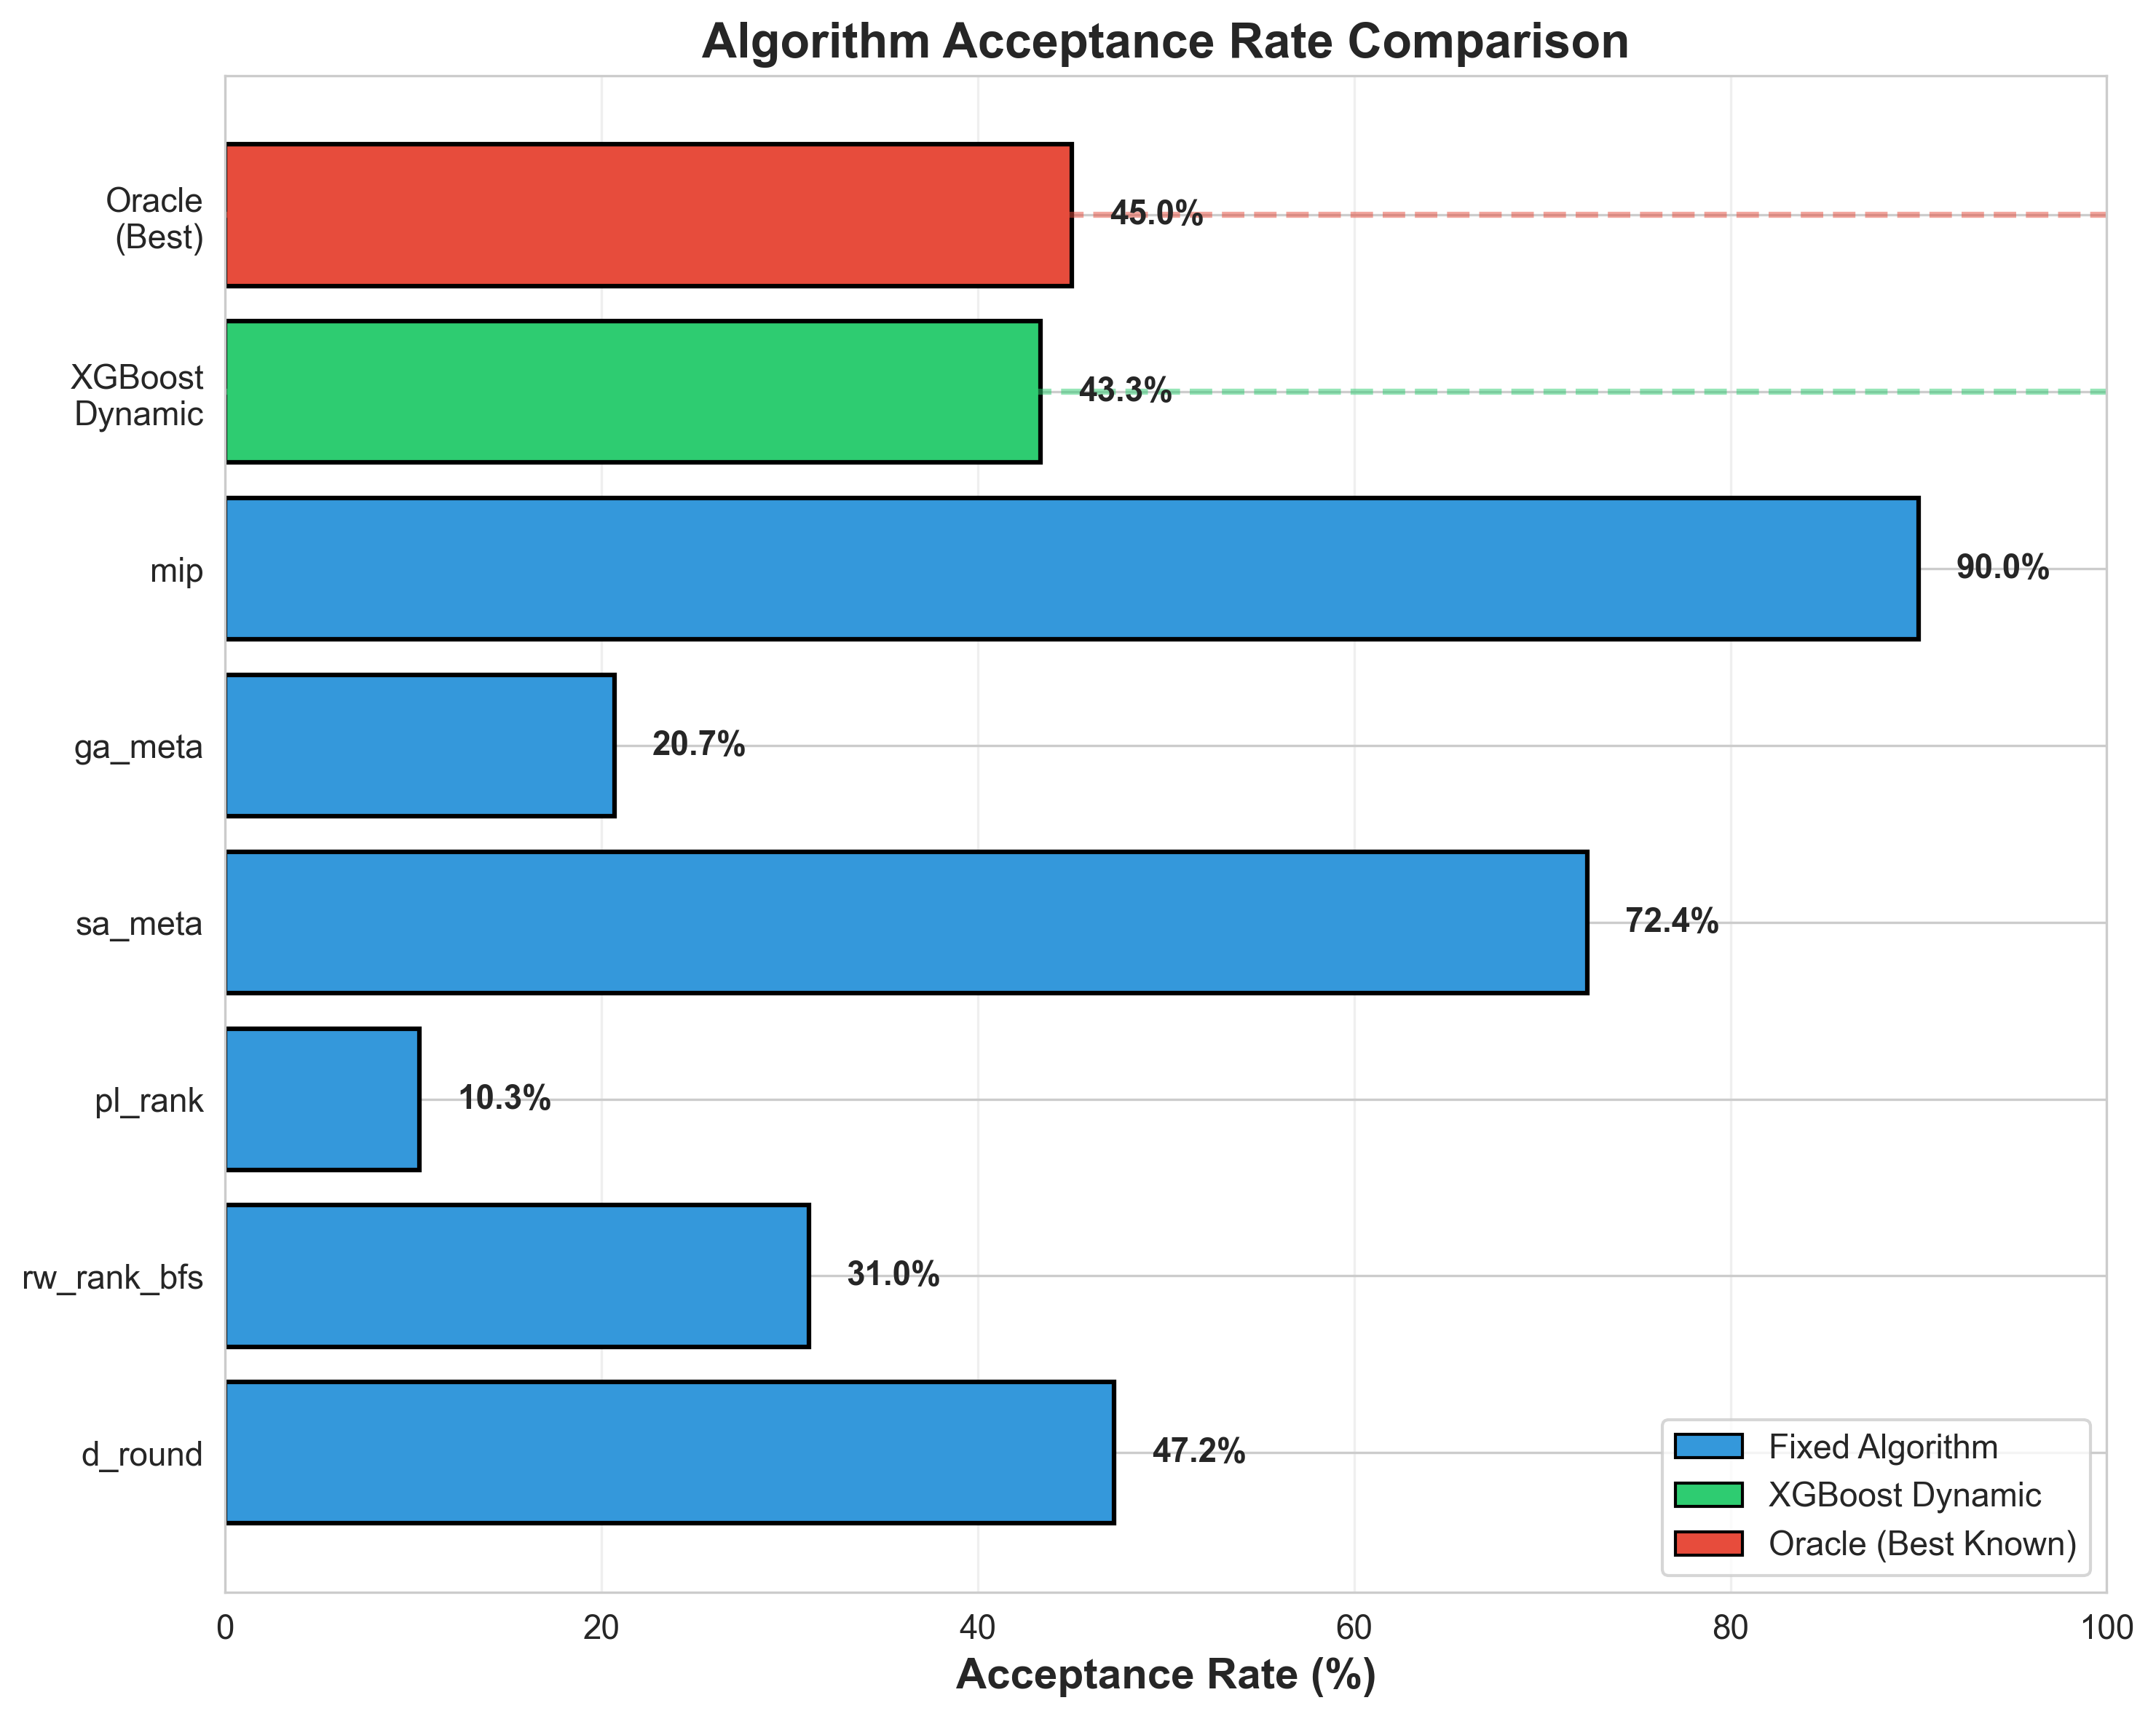
\includegraphics[width=1.0\columnwidth]{acceptance_rate_comparison.png}
    \caption{Comparação de Taxa de Aceitação entre Algoritmos}
    \label{fig:acceptance_comparison}
\end{figure}

\begin{figure}[H]
    \centering
    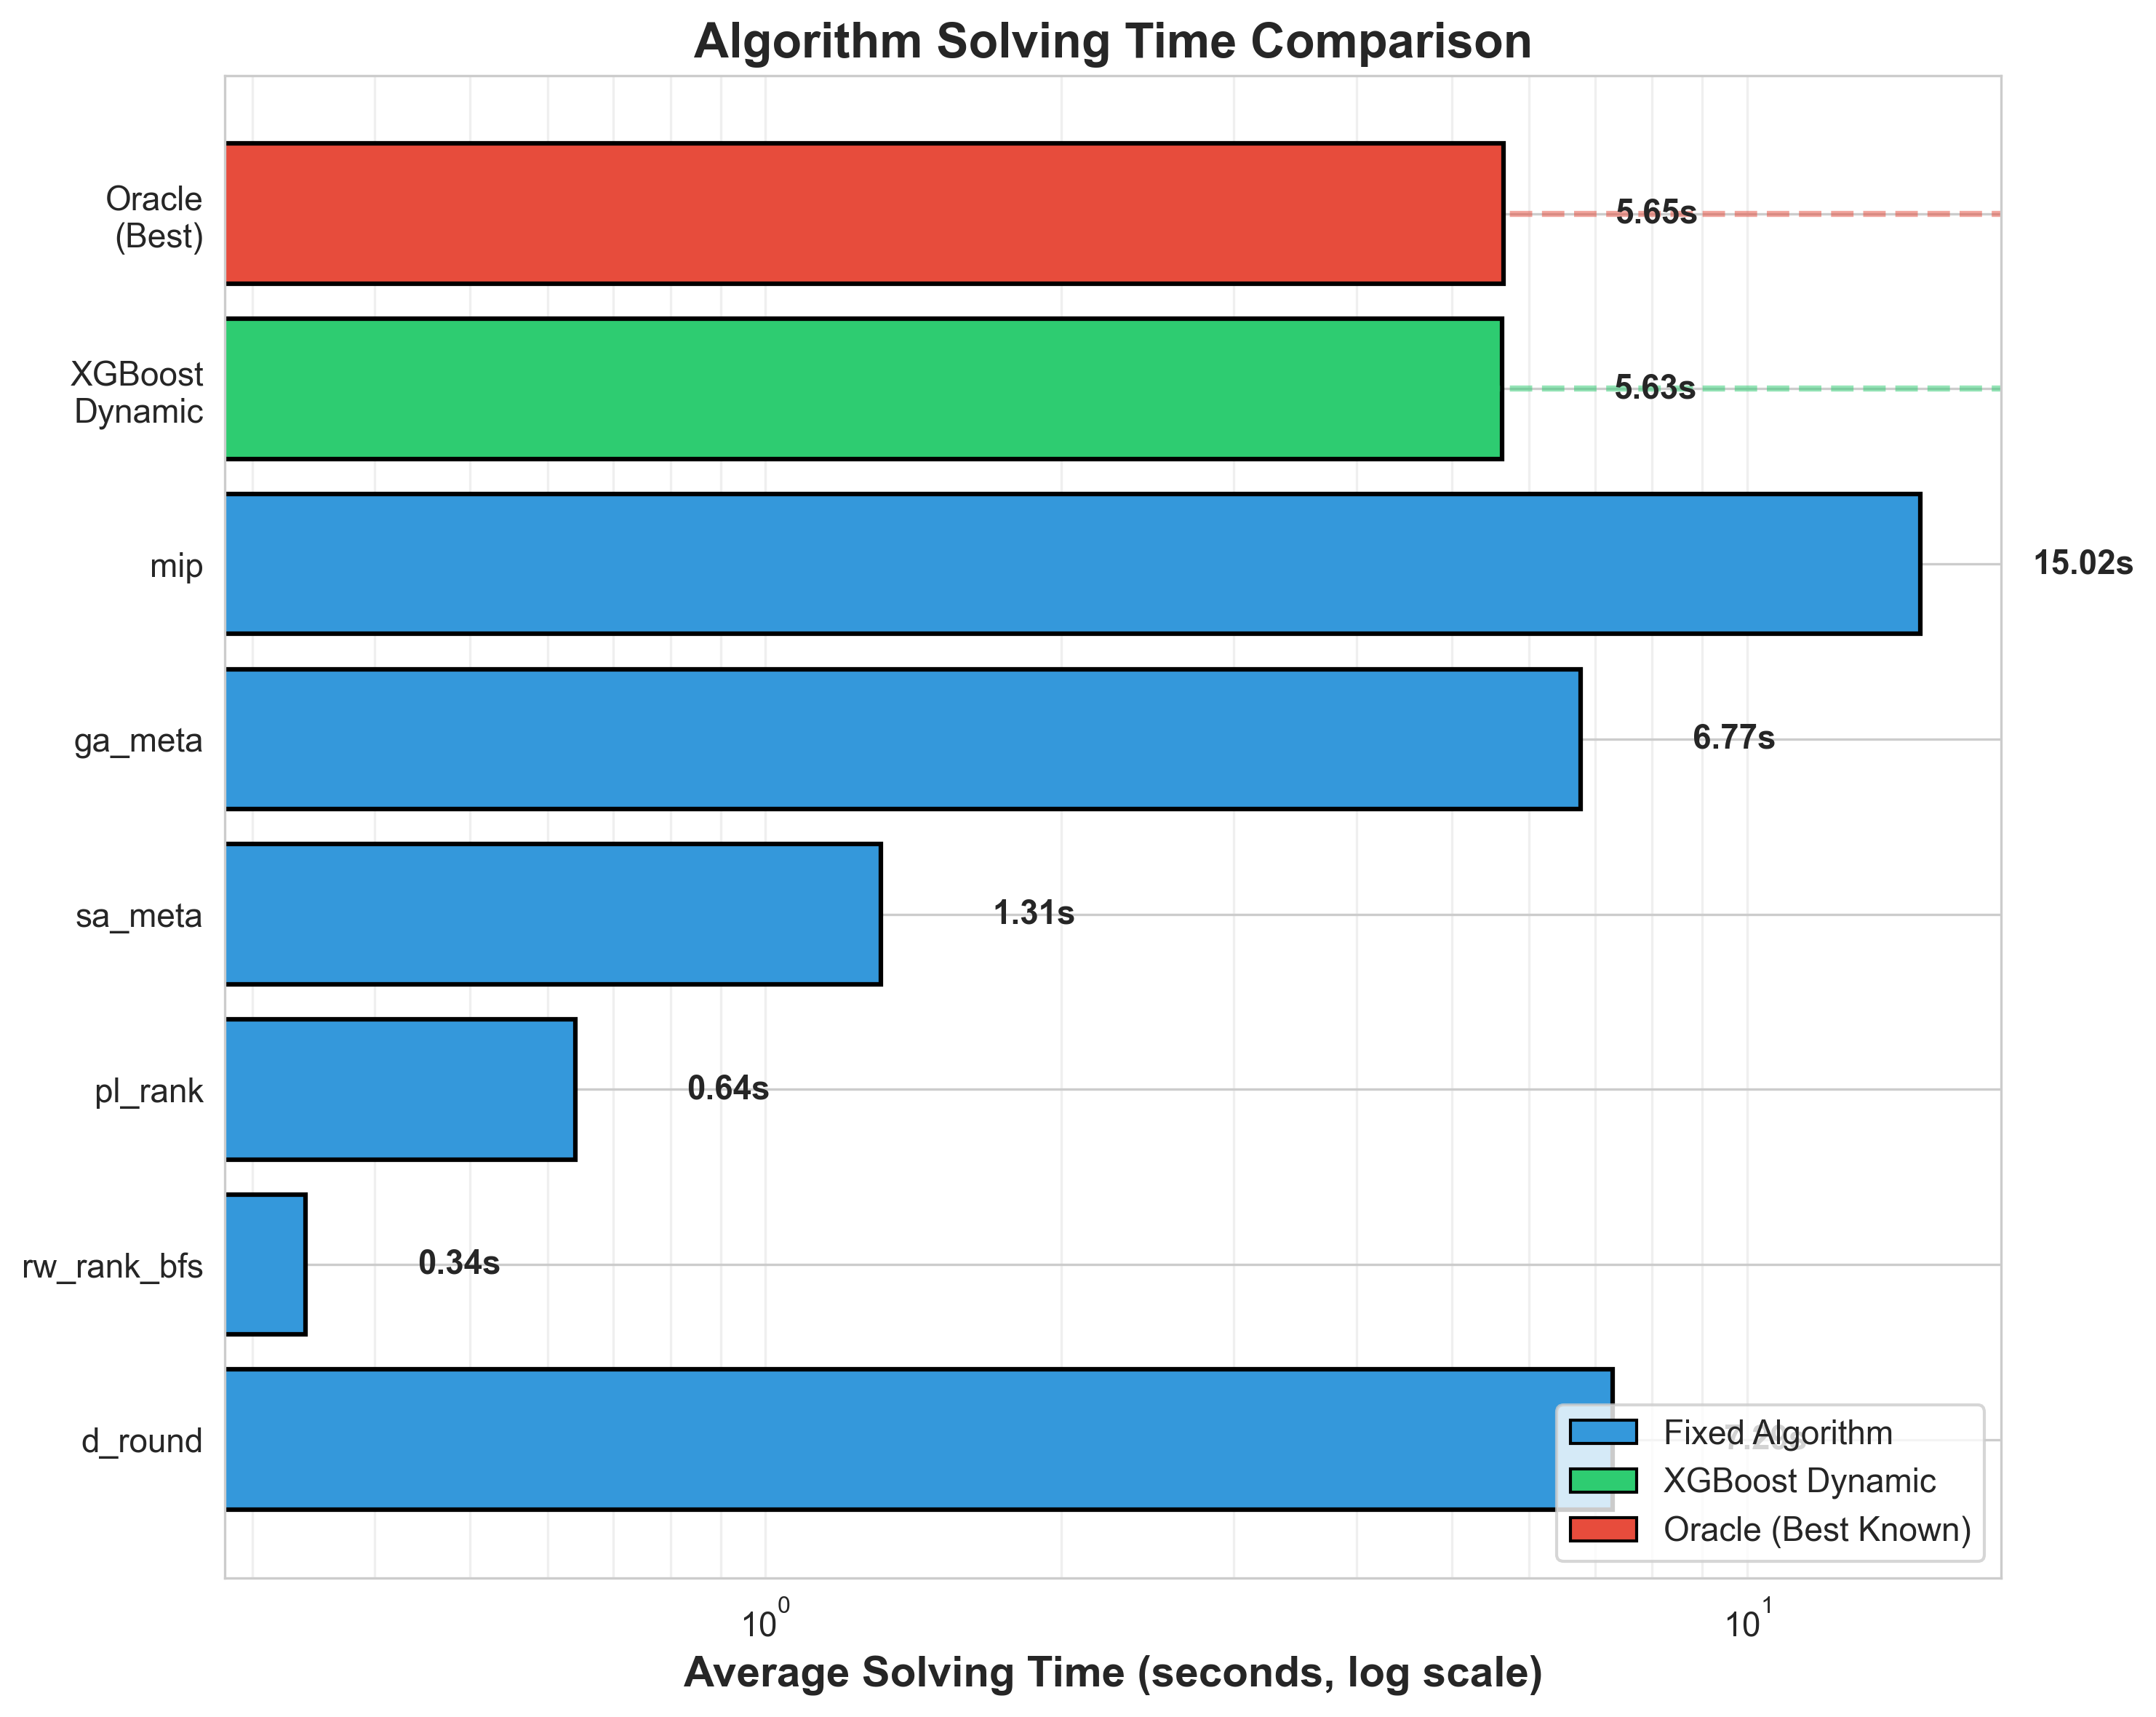
\includegraphics[width=1.0\columnwidth]{solving_time_comparison.png}
    \caption{Comparação de Tempo de Resolução entre Algoritmos}
    \label{fig:time_comparison}
\end{figure}

A Figura~\ref{fig:scatter} mostra o \textit{trade-off} entre taxa de aceitação e tempo de execução:

\begin{figure}[H]
    \centering
    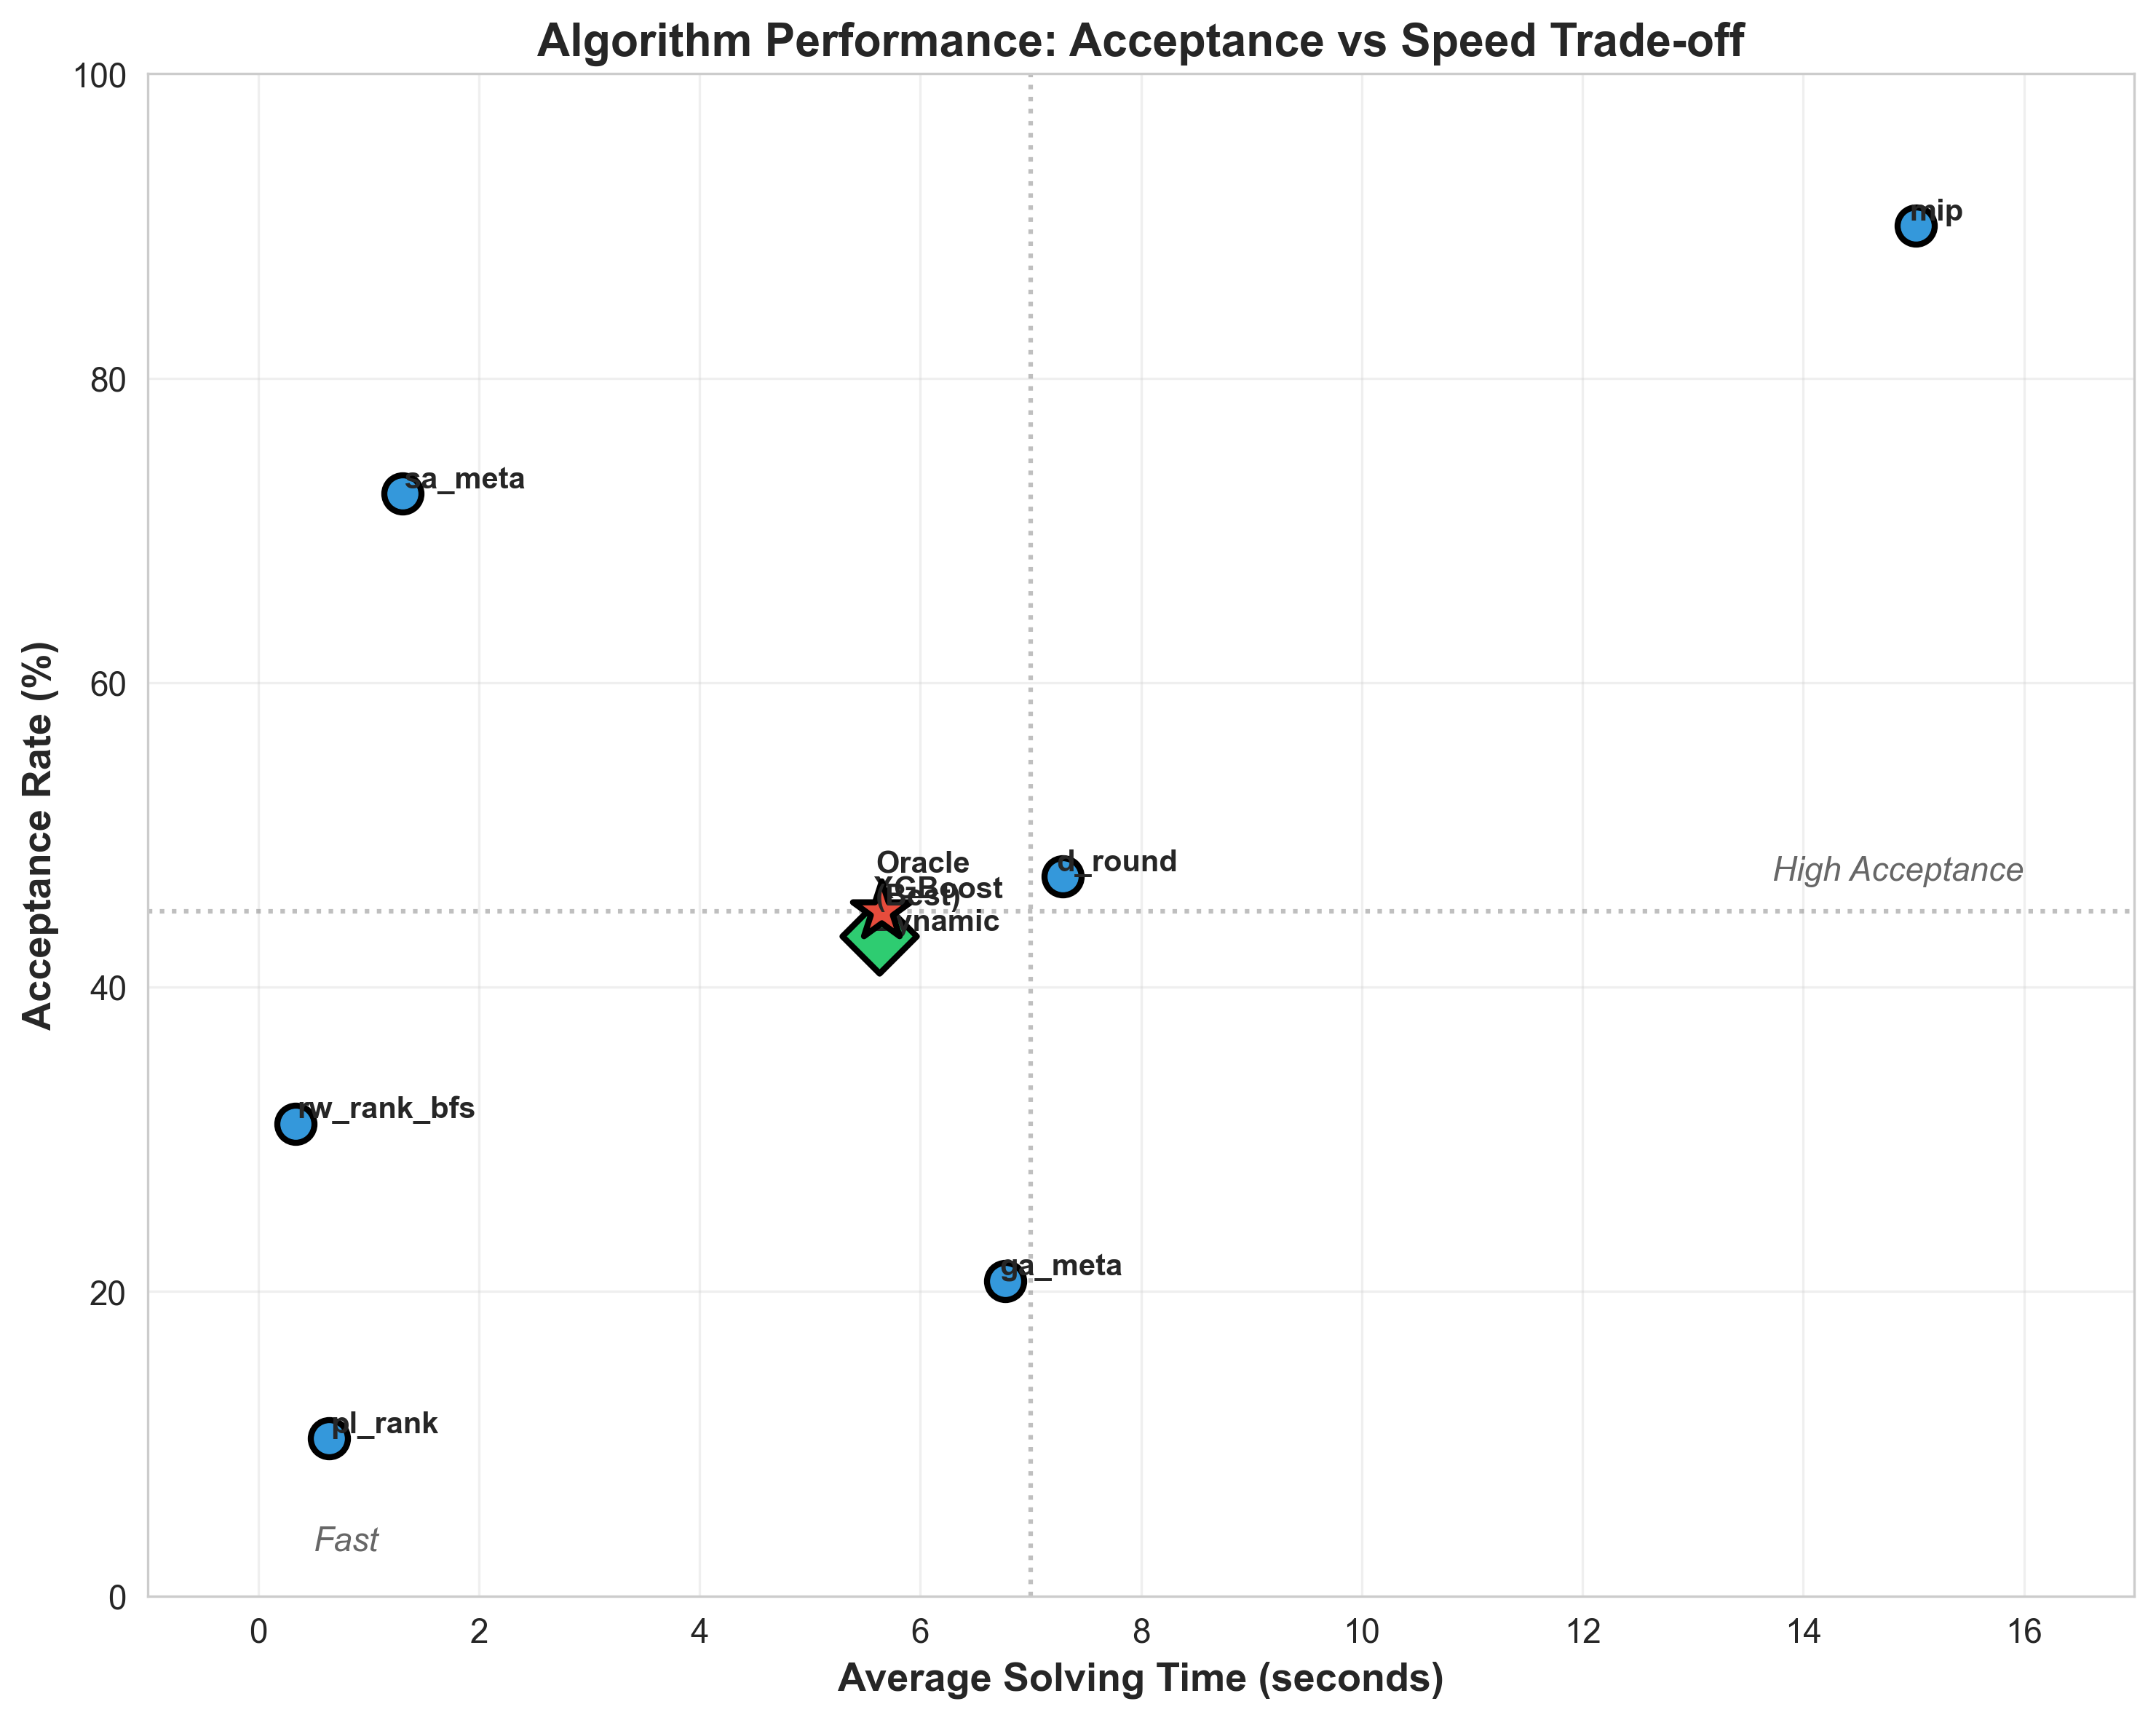
\includegraphics[width=1.0\columnwidth]{acceptance_vs_time_scatter.png}
    \caption{\textit{Trade-off} entre Taxa de Aceitação e Tempo de Execução}
    \label{fig:scatter}
\end{figure}

\subsection{Análise de Resultados}

\textbf{Desempenho Quase Ótimo}: O \textit{XGBoost} alcança 43,33\% de taxa de aceitação, apenas 1,67 pontos percentuais abaixo do oráculo teórico (45,00\%). Este pequeno \textit{gap} demonstra que o modelo aprende efetivamente a estratégia de seleção quase ótima, mesmo sem conhecimento perfeito do futuro.

\textbf{\textit{Trade-off} Equilibrado}: Enquanto MIP alcança a maior taxa de aceitação (90\%), seu tempo médio de 15,02s é 2,7× mais lento que \textit{XGBoost}. Por outro lado, \textit{RW-Rank-BFS} é o mais rápido (0,34s) mas com taxa de aceitação pobre (31,03\%). O \textit{XGBoost} oferece um meio-termo prático com 5,63s e 43,33\% de aceitação.

\textbf{Superação de \textit{Baselines}}: O seletor dinâmico supera quatro dos seis algoritmos \textit{baseline} individuais (\textit{RW-Rank-BFS}, \textit{GA-Meta}, \textit{PL-Rank} e \textit{D-Round}), demonstrando que a seleção adaptativa combina efetivamente os pontos fortes de múltiplos algoritmos.

\textbf{Limitações}: O \textit{XGBoost} não supera métodos especializados de alto desempenho como MIP (90\%) e \textit{SA-Meta} (72,41\%).

\textbf{Impacto das \textit{Features} Principais}: A análise de importância revela que tamanho relativo da VNR (49,15\%) e topologia (31,33\%) são os fatores críticos.
O tamanho relativo determina quando usar algoritmos exatos versus heurísticas rápidas, enquanto a topologia indica qual estratégia de mapeamento é mais adequada.
Por exemplo, VNRs pequenas em topologias \textit{Fat-Tree} podem beneficiar de heurísticas conscientes de estrutura hierárquica, enquanto VNRs grandes em topologias \textit{Tree} podem requerer métodos exatos.

\textbf{Eficiência Computacional}: O \textit{overhead} de predição do \textit{XGBoost} é negligenciável (menos que 0,01s), tornando a abordagem prática para uso em produção. O tempo médio de 5,63s é dominado pela execução do algoritmo VNE selecionado, não pela fase de predição.

\subsection{Discussão}

Os resultados demonstram a viabilidade de seleção dinâmica de algoritmos VNE usando \textit{XGBoost}. A alta acurácia de classificação (93,33\%) traduz-se em desempenho quase ótimo no mundo real, com apenas 1,67\% de \textit{gap} do oráculo. A análise de importância de \textit{features} fornece \textit{insights} interpretáveis: topologia e tamanho relativo da VNR direcionam as decisões de seleção.

No entanto, o desbalanceamento de classes permanece como desafio. Classes raras como MIP e \textit{GA-Meta} têm representação insuficiente, limitando a capacidade do modelo de aprender suas regiões de aplicabilidade. Trabalhos futuros devem focar em estratégias de coleta de dados balanceada, possivelmente através de amostragem dirigida ou geração sintética de VNRs.

Além disso, propostas seguintes podem comparar o seletor de algoritmo proposto com algoritmos de aprendizado por reforço, como \textit{FlagVNE}~\cite{ijcai-2024-flagvne} e \textit{HRL-ACRA} \cite{tsc-2023-hrl-acra}, que utilizam aprendizado por reforço hierárquico para alocação de recursos em redes virtuais. Tais comparações permitiriam avaliar se abordagens de seleção de algoritmos baseadas em aprendizado supervisionado oferecem vantagens em termos de eficiência computacional e qualidade de solução em relação a métodos de aprendizado por reforço fim-a-fim.

A abordagem proposta é complementar a trabalhos existentes em algoritmos VNE. Ao invés de desenvolver um novo algoritmo único, são combinados inteligentemente métodos existentes. Esta estratégia de "conjunto de algoritmos" é conceitualmente similar a \textit{ensemble} de modelos em \textit{machine learning}, nos quais múltiplos modelos fracos combinam-se em um forte.

\section{Conclusão}
\label{sec:Conclusion}

Foi proposta e avaliada uma abordagem inovadora para \textit{Virtual Network Embedding} que utiliza \textit{XGBoost} para selecionar dinamicamente o algoritmo mais apropriado para cada requisição de rede virtual. Através de experimentação com oito mil VNRs únicas, sete algoritmos VNE e duas topologias de \textit{datacenter}, foi demonstrado que a seleção adaptativa de algoritmos alcança desempenho quase ótimo, ficando apenas 1,67\% abaixo do limite teórico superior.

\subsection{Principais Contribuições}

\textbf{Metodologia de Seleção Dinâmica}: Foi desenvolvido um \textit{framework} completo que inclui geração de \textit{datasets} diversificados, engenharia de \textit{features}, otimização de hiperparâmetros via \textit{Grid Search} e avaliação contra múltiplos \textit{baselines}.

\textbf{Alta Acurácia de Predição}: O modelo \textit{XGBoost} alcança 93,33\% de acurácia e \textit{F1-score} ponderado de 92,36\%, demonstrando que características da VNR e estado da rede física são suficientes para predizer o melhor algoritmo.

\textbf{Desempenho Prático}: Em simulação de uso real, o seletor dinâmico alcança 43,33\% de taxa de aceitação com tempo médio de 5,63s, superando quatro dos seis algoritmos \textit{baseline} e oferecendo \textit{trade-off} equilibrado entre qualidade e velocidade.

\textbf{Intuições Interpretáveis}: Análise de importância de \textit{features} revela que tamanho relativo da VNR (49,15\%) e topologia (31,33\%) são os fatores dominantes, representando 80,48\% da importância total, fornecendo entendimento interpretável do processo de decisão.

\textbf{Reprodutibilidade}: Todo código fonte, \textit{datasets}, modelos treinados e \textit{scripts} de análise foram documentados e organizados para facilitar reprodução e extensão do trabalho.

\subsection{Limitações}

\textbf{Cobertura de Topologias}: O modelo foi treinado apenas em duas topologias (\textit{Tree} e \textit{Fat-Tree}). Generalização para outras estruturas de rede (GEANT, WX100, topologias reais de ISPs) requer coleta adicional de dados.

\textbf{\textit{Gap} de Desempenho}: Embora o \textit{XGBoost} (43,33\%) supere vários \textit{baselines}, algoritmos especializados como MIP (90\%) e \textit{SA-Meta} (72,41\%) ainda apresentam taxas de aceitação superiores.
A seleção dinâmica não substitui completamente o melhor algoritmo individual, mas equilibra relativamente às métricas como tempo de encaixe.

\textbf{Características Estáticas}: As \textit{features} atuais capturam apenas estado instantâneo da rede. Histórico temporal, padrões de chegada de VNRs e previsão de carga futura poderiam melhorar as decisões de seleção.

\subsection{Trabalhos Futuros}

\textbf{Aprendizado \textit{Online}}: Implementar atualização contínua do modelo conforme novas VNRs são processadas. Isto permitiria adaptação a mudanças no padrão de requisições e evolução da rede física.

\textbf{Amostragem Balanceada}: Desenvolver estratégias de coleta de dados que garantam representação adequada de todos os algoritmos, possivelmente através de geração de VNRs sintéticas especificamente desenhadas para favorecer algoritmos raros.

\textbf{Expansão de Topologias}: Treinar modelos em topologias diversas incluindo GEANT, WX100, topologias de ISPs reais e redes de \textit{datacenter} de larga escala. \textit{Transfer learning} poderia facilitar adaptação entre topologias.

\textbf{Otimização Multi-Objetivo}: Estender o modelo para considerar explicitamente múltiplos objetivos (aceitação, tempo, custo energético, SLA) através de formulação multi-objetivo ou \textit{ensemble} de modelos especializados.

\textbf{\textit{Deep Learning}}: Investigar arquiteturas de redes neurais profundas, especialmente \textit{Graph Neural Networks} que podem explorar diretamente a estrutura topológica de VNRs e redes físicas.

\textbf{Seleção baseada em confiança}: Utilizar probabilidades de predição do \textit{XGBoost} para recorrer ao MIP quando o modelo está incerto, combinando velocidade de heurísticas com otimalidade de métodos exatos.

\textbf{Considerações de Energia e SLA}: Incorporar restrições de consumo energético e \textit{Service Level Agreements} como \textit{features} adicionais e objetivos de otimização, tornando a seleção consciente de sustentabilidade e requisitos contratuais.

%===================================================================


\bibliographystyle{IEEEtran}
\bibliography{references}

\end{document}